\section{Projected Bellman Error}
\label{sec:bellman_error}

This section explains several key ideas in Reinforcement Learning and Approximate Dynamic Programming:


In approximate dynamic programming or reinforcement learning, $v$ may lie in a restricted function space (e.g., a parametric class of value functions). Hence, we cannot always solve 
\[
(I - P')\,v = r - g\,\mathbf{1}
\]
exactly. Instead, we use a \emph{projection} operator $\mathbb{P}$ that projects any function onto our approximation space. Thus, the \emph{projected Bellman error} (PBE) is defined as:
\[
\text{PBE}(v) 
\;=\; \mathbb{P}\Bigl[(r - g\,\mathbf{1}) + P'\,v\Bigr] \;-\; v.
\]
This quantity indicates how close the projected Bellman update $\mathbb{P}[\mathbb{B}v]$ is to $v$, where the Bellman operator is given by
\[
\mathbb{B}v \;\equiv\; r - g\,\mathbf{1} \;+\; P'v.
\]
Minimizing the PBE is a common strategy in methods such as LSTD, where we seek a parameterized value function $\hat{v}(w)$ that is as close as possible (in a projected sense) to the Bellman update.

\subsubsection{Norm-Based View of PBE}
A common way to quantify the PBE is via a weighted $\ell_2$-norm (often using the stationary distribution $p^*(s)$ as weights). Let
\[
\Delta v(s) \;=\; \hat{v}(w)(s) \;-\; \mathbb{P}\bigl[\mathbb{B}\,\hat{v}(w)\bigr](s).
\]
Then, the PBE can be measured as:
\[
e_{\mathrm{PB}}
\;=\;
\bigl\lVert \Delta v \bigr\rVert_{p^*}^2
\;=\;
\sum_{s} p^*(s)\,\bigl[\Delta v(s)\bigr]^2
\;=\;
\mathbb{E}_{s \sim p^*}\bigl[\Delta v(s)^2\bigr].
\]
When $e_{\mathrm{PB}} = 0$, it implies that $\hat{v}(w)$ is a fixed point of the projected Bellman operator, i.e., $\hat{v}(w) = \mathbb{P}[\mathbb{B}\,\hat{v}(w)]$.

\subsection{Why It Does Not Involve the True Value}
A key point is that we do \emph{not} need the \emph{true} value function $v^*$ to measure or minimize the Bellman error equation (or the projected Bellman error). Instead, we only need:
\begin{itemize}
    \item Observations of $(s, r(s), s')$ transitions (in model-free settings), or
    \item A model for the reward and transition probabilities (in model-based settings).
\end{itemize}
From these, we can construct the Bellman operator $\mathbb{B}$ (or an empirical version of it) and compare $\mathbb{B}v$ to $v$. This approach is stable because it relies on the \emph{self-consistency} property of the Bellman equation rather than on direct knowledge of $v^*$.

\subsection{Temporal Difference Error Connection}
Methods like \emph{Temporal Difference (TD) learning} effectively estimate the Bellman error equation incrementally. A TD update can be viewed as trying to drive the quantity
\[
\delta_t 
= r_t - g + v(s_{t+1}) - v(s_t)
\]
to zero over time, which corresponds to making $v$ satisfy the Bellman equation in expectation.

\subsection{Geometric Interpretation in Parameter Space}

\begin{figure}[ht]
\centering
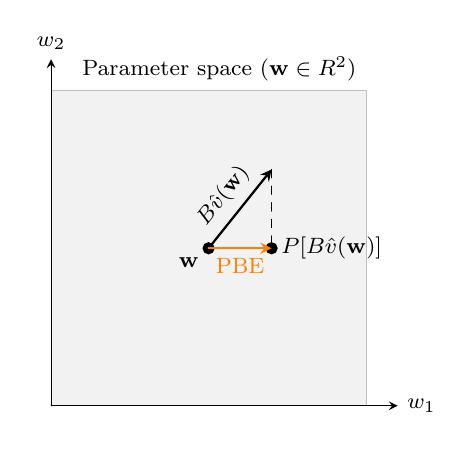
\begin{tikzpicture}[scale=2, >=stealth, line join=round, line cap=round]
    
    % Light gray square representing the 2D parameter space
    \draw[fill=gray!10, draw=gray!50] (0,0) rectangle (2,2);
    \node[above left] at (2,2) {\footnotesize Parameter space ($\mathbf{w}\in\mathbb{R}^2$)};
    
    % Axes in the parameter space
    \draw[->] (0,0) -- (2.2,0) node[right] {\footnotesize $w_1$};
    \draw[->] (0,0) -- (0,2.2) node[above] {\footnotesize $w_2$};
    
    % Current parameter vector w in the plane
    \coordinate (W) at (1,1);
    \draw[fill] (W) circle (1pt) node[below left] {\footnotesize $\mathbf{w}$};
    
    % Point representing the Bellman update of v at w, outside the parameter space
    \coordinate (BvWout) at (1.4,1.5);
    \draw[->, thick] (W) -- (BvWout)
         node[midway,sloped,above] {\footnotesize $\mathbb{B}\hat{v}(\mathbf{w})$};
    
    % Projection of Bv(w) back into the parameter space
    \coordinate (PiBvW) at (1.4,1.0);
    \draw[fill] (PiBvW) circle (1pt)
         node[right] {\footnotesize $\mathbb{P}[\mathbb{B}\hat{v}(\mathbf{w})]$};
    
    % Dashed line showing the projection from the Bellman update to its projection
    \draw[dashed] (BvWout) -- (PiBvW);
    
    % Arrow from w to the projection, indicating the Projected Bellman Error (PBE)
    \draw[->, thick, orange] (W) -- (PiBvW)
         node[midway,sloped,below] {\footnotesize PBE};
    
\end{tikzpicture}
\caption{Conceptual illustration of the geometric interpretation in parameter space. The light gray square represents the 2D parameter space where $\mathbf{w}$ resides. Applying the Bellman operator $\mathbb{B}$ to $\hat{v}(\mathbf{w})$ can yield a value function outside the representable space (point $\mathbb{B}\hat{v}(\mathbf{w})$). The projection operator $\mathbb{P}$ then maps it back into the parameter space (point $\mathbb{P}[\mathbb{B}\hat{v}(\mathbf{w})]$). The orange arrow (labeled PBE) shows the difference between the current value function and its projected Bellman update.}
\label{fig:param_space}
\end{figure}

\paragraph{Explanation of the Diagram:}
\begin{itemize}
    \item \textbf{Parameter Space:} The light gray square represents the 2D parameter space, with axes $w_1$ and $w_2$. Every point in this space corresponds to a set of parameters $\mathbf{w}$ defining the approximate value function $\hat{v}(\mathbf{w})$.
    \item \textbf{Current Parameter Vector:} The point labeled $\mathbf{w}$ (located at $(1,1)$ in this example) is our current estimate in the parameter space.
    \item \textbf{Bellman Operator Application:} The arrow from $\mathbf{w}$ to the point labeled $\mathbb{B}\hat{v}(\mathbf{w})$ represents the application of the Bellman operator. This update may move the value function outside the representable parameter space.
    \item \textbf{Projection Operator:} The dashed line and the point $\mathbb{P}[\mathbb{B}\hat{v}(\mathbf{w})]$ indicate that we use a projection operator $\mathbb{P}$ to map the Bellman update back into our parameter space.
    \item \textbf{Projected Bellman Error (PBE):} The orange arrow from $\mathbf{w}$ to $\mathbb{P}[\mathbb{B}\hat{v}(\mathbf{w})]$ represents the Projected Bellman Error. Minimizing this error is key to ensuring that our approximate value function is as close as possible to being a fixed point of the projected Bellman operator.
\end{itemize}

\subsection{Projection Operator \texorpdfstring{$\mathbb{P}$}{P}}

Suppose we have:
\[
\text{feature matrix: } F \in \mathbb{R}^{|S|\times k}, 
\quad
\text{diagonal weighting: } D_{p^*} \in \mathbb{R}^{|S|\times |S|}.
\]
Here, $|S|$ is the number of states (or samples), and each row of $F$ is a feature vector $f(s)^T$ for state $s$. The matrix $D_{p^*}$ is diagonal with entries $p^*(s)$, representing a stationary distribution or weighting over states.

We wish to define a \emph{projection} operator
\[
\mathbb{P}: \mathbb{R}^{|S|} \;\to\; \text{Col}(F),
\]
where $\text{Col}(F)$ is the column space spanned by $F$. The projection is taken under the $\ell_2$-norm weighted by $D_{p^*}$, namely
\[
\|x\|_{D_{p^*}}^2 \;=\; x^T\,D_{p^*}\,x.
\]
Formally, for any vector $v \in \mathbb{R}^{|S|}$, we define
\[
\mathbb{P}(v) \;=\; \arg\min_{x \in \text{Col}(F)} \;\|v - x\|_{D_{p^*}}^2.
\]
Since $x \in \text{Col}(F)$ can be written as $x = Fw$ for some $w \in \mathbb{R}^k$, the problem becomes:
\[
\mathbb{P}(v) 
\;=\; \arg\min_{Fw} \;\|v - Fw\|_{D_{p^*}}^2.
\]
We can solve for $w$ by expanding and taking derivatives.

\paragraph{Step-by-Step Derivation:}

\begin{enumerate}
    \item \textbf{Rewrite the objective:}
    \[
    \|v - Fw\|_{D_{p^*}}^2 
    \;=\; (v - Fw)^T\,D_{p^*}\,(v - Fw).
    \]
    
    \item \textbf{Take the gradient with respect to $w$:}
    \[
    \frac{\partial}{\partial w} 
    \bigl[(v - Fw)^T\,D_{p^*}\,(v - Fw)\bigr]
    \;=\;
    -2\,F^T\,D_{p^*}\,(v - Fw).
    \]
    Setting this to zero for optimality yields:
    \[
    F^T\,D_{p^*}\,(v - Fw) \;=\; 0 
    \quad\Longrightarrow\quad
    F^T\,D_{p^*}\,F\,w \;=\; F^T\,D_{p^*}\,v.
    \]
    
    \item \textbf{Solve for $w$:}
    \[
    w^* 
    \;=\; \bigl(F^T\,D_{p^*}\,F\bigr)^{-1}\,F^T\,D_{p^*}\,v.
    \]
    
    \item \textbf{Hence, the projection of $v$:}
    \[
    \mathbb{P}(v)
    \;=\; F\,w^*
    \;=\; F\,\bigl(F^T\,D_{p^*}\,F\bigr)^{-1}\,F^T\,D_{p^*}\,v.
    \]
\end{enumerate}

Therefore, the projection operator $\mathbb{P}$ onto the column space of $F$ under the $D_{p^*}$-weighted norm is
\[
\boxed{
\mathbb{P} 
\;=\; 
F\,\bigl(F^T\,D_{p^*}\,F\bigr)^{-1}\,F^T\,D_{p^*}.
}
\]
In other words, for any vector $v$, $\mathbb{P}(v)$ is given by the above formula.

\subsection{Deriving \texorpdfstring{$w^*$}{w*} to Minimize the Projected Bellman Error}

Next, consider a \emph{linear} approximate value function:
\[
\hat{v}(w) \;=\; F\,w.
\]
The \emph{Projected Bellman Error} (PBE) can be defined (in squared norm) as
\[
e_{\mathrm{PB}}(w)
\;=\;
\bigl\|
\hat{v}(w) 
\;-\;
\mathbb{P}\bigl[\mathbb{B}\,\hat{v}(w)\bigr]
\bigr\|_{D_{p^*}}^2,
\]
where $\mathbb{B}$ is the Bellman operator, e.g.,
\[
\mathbb{B}\,\hat{v}(w)
\;=\;
r \;-\; g\,\mathbf{1}
\;+\;
P'\,\bigl(F\,w\bigr).
\]
We want:
\[
w^*
\;=\;
\arg\min_{w}
\;e_{\mathrm{PB}}(w).
\]

\paragraph{Outline of the Solution:}
\begin{itemize}
    \item \textbf{Apply $\mathbb{P}$:} 
    \[
    \mathbb{P}\bigl[\mathbb{B}\,\hat{v}(w)\bigr]
    \;=\;
    F\,(F^T D_{p^*} F)^{-1} F^T\,D_{p^*}\,\bigl(r - g\,\mathbf{1} + P'\,F\,w\bigr).
    \]
    
    \item \textbf{Compute the difference:}
    \[
    \hat{v}(w) 
    \;-\;
    \mathbb{P}\bigl[\mathbb{B}\,\hat{v}(w)\bigr]
    \;=\;
    F\,w
    \;-\;
    F\,(F^T D_{p^*} F)^{-1} F^T\,D_{p^*}\,\bigl(r - g\,\mathbf{1} + P'\,F\,w\bigr).
    \]
    
    \item \textbf{Square under $D_{p^*}$:}
    \[
    e_{\mathrm{PB}}(w)
    \;=\;
    \bigl\|
    F\,w
    \;-\;
    F\,(F^T D_{p^*} F)^{-1} F^T\,D_{p^*}\,\bigl(r - g\,\mathbf{1} + P'\,F\,w\bigr)
    \bigr\|_{D_{p^*}}^2.
    \]
    One can then take the gradient with respect to $w$ and set it to zero. 
    Under suitable assumptions (like invertibility of $(F^T D_{p^*} (I - P') F)$), 
    the resulting $w^*$ often matches the well-known LSTD solution:
    \[
    w^*
    \;=\;
    \bigl(F^T\,D_{p^*}\,\bigl(I - P'\bigr)\,F\bigr)^{-1}
    F^T\,D_{p^*}\,\bigl(r - g\,\mathbf{1}\bigr).
    \]
\end{itemize}

\paragraph{Interpretation.}
\begin{itemize}
    \item \emph{Projection}: We only need to operate in the subspace spanned by $F$. Instead of trying to match the Bellman operator $\mathbb{B}\hat{v}(w)$ exactly, we \emph{project} it back into $\text{Col}(F)$.
    \item \emph{Weighted Norm}: The diagonal matrix $D_{p^*}$ imposes a weighting, typically corresponding to a stationary distribution over states. States with higher probability mass get higher influence in the error measure.
    \item \emph{Minimizing PBE}: Solving $\arg\min_w e_{\mathrm{PB}}(w)$ yields $w^*$ that best satisfies the Bellman equation in the projected sense. This is precisely the principle behind LSTD and related least-squares policy/value evaluation methods.
\end{itemize}

\noindent
\textbf{Final Summary.}  
The key formulas are:
\[
\boxed{
\mathbb{P}(v) 
= 
F \,\bigl(F^T\,D_{p^*}\,F\bigr)^{-1}\,F^T\,D_{p^*}\,v,
\quad
w^*
= 
\arg\min_{w}\,
\bigl\|\,
F w
\;-\;
\mathbb{P}\bigl[\mathbb{B}(F w)\bigr]
\bigr\|_{D_{p^*}}^2.
}
\]
They show how the projection operator arises from a simple least-squares argument and how, in turn, one can derive the optimal parameter vector $w^*$ by minimizing the Projected Bellman Error.

\subsection{Taking the Gradient and Finding \texorpdfstring{$w^*$}{w*}}

When we want to find a parameter vector \(w^*\) that minimizes a function \(e_{\mathrm{PB}}(w)\)
(such as the Projected Bellman Error in a linear approximation setting), we typically follow these steps:

\begin{enumerate}
    \item \textbf{Compute the gradient:} 
    \[
    \nabla_w \, e_{\mathrm{PB}}(w).
    \]
    \item \textbf{Set the gradient to zero:} 
    \[
    \nabla_w \, e_{\mathrm{PB}}(w) \;=\; 0.
    \]
    \item \textbf{Solve for \(w\):} 
    The solution \(\widehat{w}\) that satisfies \(\nabla_w \, e_{\mathrm{PB}}(\widehat{w}) = 0\)
    is a \emph{critical point}. Under suitable convexity conditions (or in least-squares problems),
    this critical point is a global minimum, which we denote by \(w^*\).
\end{enumerate}

Intuitively, at the minimum of a differentiable function, the slope (or gradient) is zero. This is
visualized in a simple 1D schematic in Figure~\ref{fig:grad_zero}, where the horizontal axis 
represents the parameter \(w\), and the vertical axis represents the error function \(e\). 

\begin{figure}[ht]
\centering
\begin{tikzpicture}[>=stealth, scale=1.2, line cap=round, line join=round]
    % Axes
    \draw[->] (-0.3,0) -- (5,0) node[right] {\footnotesize $w$};
    \draw[->] (0,-0.3) -- (0,3) node[above] {\footnotesize $e$};

    % Parabola
    \draw[domain=0.4:4.4, smooth, thick, blue] 
        plot (\x, {0.4+0.5*(\x-2.4)^2});
    
    % Mark the minimum point
    \coordinate (wStar) at (2.4,0.4);
    \draw[fill=red] (wStar) circle (1.5pt);
    \node[below] at (wStar) {\footnotesize $w^*$};

    % Dashed line from wStar down to x-axis
    \draw[dashed] (wStar) -- ++(0,-0.4);

    % Annotations
    \node[below left] at (0,0) {\footnotesize $(0,0)$};
    \node[right, text width=4.2cm] at (2.7,2.2)
    {\footnotesize \textcolor{blue}{\emph{Error function} $e_{\mathrm{PB}}(w)$}};
\end{tikzpicture}
\caption{A conceptual 1D illustration of minimizing an error function $e$ by setting its gradient to zero. 
At the minimum $w^*$, the slope (or derivative) is zero.}
\label{fig:grad_zero}
\end{figure}

\paragraph{Key Takeaways:}
\begin{itemize}
    \item Setting \(\nabla_w \, e_{\mathrm{PB}}(w) = 0\) is the standard procedure to find a minimum in differentiable optimization.
    \item In the context of LSTD or other least-squares methods, solving this equation often yields a \emph{closed-form} expression for \(w^*\).
    \item Graphically, a zero gradient corresponds to the point where the error curve has zero slope (the bottom of a parabola in a 1D schematic).
\end{itemize}
